\documentclass[12pt,twocolumn]{article}
\usepackage[margin=1.5cm]{geometry}
\usepackage{amsmath}
\usepackage{graphicx}
\usepackage{hyperref}
\usepackage{sectsty}
\title{Midterm 1}
\author{Prof. Jordan C. Hanson}
\sectionfont{\fontsize{12}{15}\selectfont}

\begin{document}
\maketitle

\section{Unit 0: Electrostatics I and II}

\noindent
\begin{enumerate}
\item A 50 gram copper wire has a net charge of 2.00 $\mu$C. What fraction of the copper’s electrons has been removed? (Each atom has 29 protons, and the atomic mass is 63.5.) \\ \vspace{2cm}
\item A test charge of +2 $\mu$C is placed halfway between a charge of +6 $\mu$C and another of +4 $\mu$C separated by 10 cm. (a) What is the magnitude of the net force on the test charge? (b) What is the direction of this force (away from or toward the +6 $\mu$C charge)? \\ \vspace{3cm}
\item What is the force on the charge located at $x=8.00$ cm in Fig. \ref{fig:e-field_1}(a) given that $q=1.00$ $\mu$C?
\begin{figure}[hb]
\centering
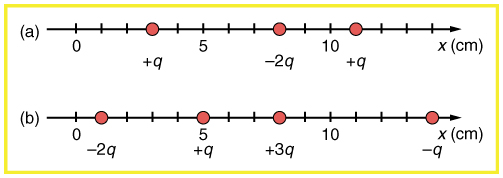
\includegraphics[width=0.49\textwidth]{e-field_1.jpeg}
\caption{\label{fig:e-field_1} Linear arrangement of charges.}
\end{figure}
\item Find the total electric field at $x=11.00$ cm in Fig. \ref{fig:e-field_1}(b). \\ \vspace{5cm}
\item Determine the direction of the force on $q$ in Fig. \ref{fig:e-field_2}, given that $q_a=q_b=+7.50$ $\mu$C and $q_c = q_d = -7.50$ $\mu$C. (b) Calculate the force on the charge $q$, given that the square is 10.0 cm on a side and $q=2.00$ $\mu$C.
\begin{figure}[hb]
\centering
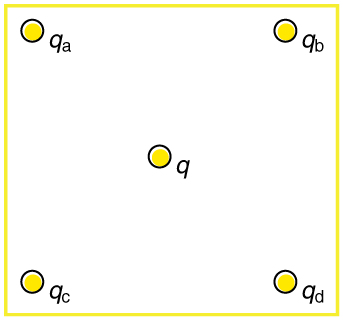
\includegraphics[width=0.25\textwidth]{e-field_2.jpeg}
\caption{\label{fig:e-field_2} 2D arrangement of charges.}
\end{figure} \vspace{4cm}
\item (a) An evacuated tube uses an accelerating voltage of 40 kV to accelerate electrons to hit a copper plate and produce x rays. Non-relativistically, what would be the maximum speed of these electrons? (b)  Show that units of V/m and N/C for electric field strength are indeed equivalent. \\ \vspace{3cm}
\item The electric field strength between two parallel conducting plates separated by 4.00 cm is $7.50 \times 10^4$ V m$^{-1}$. (a) What is $\Delta V$ between the plates? (b) The plate with the lowest potential is taken to be at zero volts. What is the potential 1.00 cm from that plate (and 3.00 cm from the other)? (c) The voltage across a membrane forming a cell wall is 80.0 mV and the membrane is 9.00 nm thick. What is the electric field strength?\footnote{The value is surprisingly large, but correct.} \\ \vspace{4cm}
\item A doubly charged ion is accelerated to an energy of 32.0 keV by the electric field between two parallel conducting plates separated by 2.00 cm. What is the electric field strength between the plates? \\ \vspace{2cm}
\item In one of the classic nuclear physics experiments at the beginning of the 20th century, an alpha particle was accelerated toward a gold nucleus, and its path was substantially deflected by the Coulomb interaction. If the energy of the doubly charged alpha nucleus was 5.00 MeV, how close to the gold nucleus (79 protons) could it come before being deflected? \\ \vspace{3cm}
\end{enumerate}

\section{Unit 1: Capacitors, Current, and DC \\ circuits}

\noindent
\begin{enumerate}
\item What capacitance is needed to store 3.00 $\mu$C of charge at a voltage of 120 V? \\ \vspace{2cm}
\item (a) What is the energy stored in the 10.0 $\mu$F capacitor of a heart defibrillator charged to $9.00\times 10^3$ V? (b) Find the amount of stored charge. (c) In open heart surgery, a much smaller amount of energy will defibrillate the heart.  What voltage is applied to the 8.00 $\mu$F capacitor of a heart defibrillator that stores 40.0 J of energy? (d) Find the amount of stored charge. \\ \vspace{5cm}
\end{enumerate}

\section{Unit 2: DC circuits with resistors in \\ series and parallel, RC circuits}

\noindent
\begin{enumerate}
\item t
\end{enumerate}

\section{Unit 3: Magnetism I}

\noindent
\begin{enumerate}
\item t
\end{enumerate}

\end{document}